\documentclass{beamer}
 
\usetheme{Madrid}
\usepackage{listings}
\lstset{numbers=left,
	xleftmargin=2em,frame=lines,
	keywordstyle=\color{blue}\bfseries,
	framexleftmargin=1.5em,
	basicstyle=\ttfamily\tiny,
	language=Java}

\usepackage{subfigure}
\usepackage{caption}
\usepackage{graphicx}

 
 \title[RunDroid: Recovering  CGs for Android Apps.]{RunDroid:}
 \subtitle{Recovering Execution Call Graphs for Android Applications}
 

\author[Y. Yuan, L. Xu, X. Xiao, A. Podgursk, H. Zhu] % (optional, for multiple authors)
{Yujie Yuan\inst{1} \and Lihua Xu \inst{1} \and Xusheng Xiao\inst{2} \\  \and Andy Podgurski\inst{2} \and Huibiao Zhu\inst{1}}

\institute[ECNU,CWRU] % (optional)
{
	\inst{1}%
	East China Normal University, China
	\and
	\inst{2}%
	Case Western Reserve University, USA
}

\date[ESEC/FSE 2017]
{ESEC/FSE 2017, SEPTEMBER 04 - 08}

 
\begin{document}

 \frame{\titlepage}
 
 %---------------------------------------------------------
 %This block of code is for the table of contents after
 %the title page
 \begin{frame}
 \frametitle{Table of Contents}
 \tableofcontents
\end{frame}
%---------------------------------------------------------

\section{ Why we need RunDroid}
\begin{frame}
\frametitle{Why we need RunDroid}
\textbf{Intention}\\
Tell us what happen during app running?

\textbf{Challenges in Android}
\begin{itemize}
\item Implicit callbacks
\item Lifecycle methods
\item Multi-thread communications
\end{itemize}
\textbf{Analysis tools in Android}
\begin{itemize}
	\item Static Analysis $\longrightarrow$ time \& space cost
	\item Dynamic Analysis $\longrightarrow$ time \& technique cost
\end{itemize}
%有时我们需要了解查询在执行时的具体过程
\end{frame}

\section{How RunDroid works}
\begin{frame}
\frametitle{Basic idea in RunDroid}

\textbf{RunDroid}


A tool that captures the dynamic method executions during each app running, and recovers the complete dynamic call graph to help people know what happen during app running.
\newline
\newline
\textbf{Overview}

RunDroid takes the source code of an app as input, instruments the source code, and intercepts the executions of the instrumented app to analyze message objects. After each execution, RunDroid produces a set of log files, which will be further analyzed to generate the dynamic call graph for the execution.
\newline

\begin{alertblock}{Note}
We assume we can access the code of programs.
\end{alertblock}
\end{frame}


\begin{frame}
\frametitle{RunDroid's Framework}
\framesubtitle{Three steps}
\textbf{Three steps:}

\begin{enumerate}
\item Capture application layer method calls
\item Recover method calls between app and the Android framework
\item Build dynamic call graphs\newline
\end{enumerate}
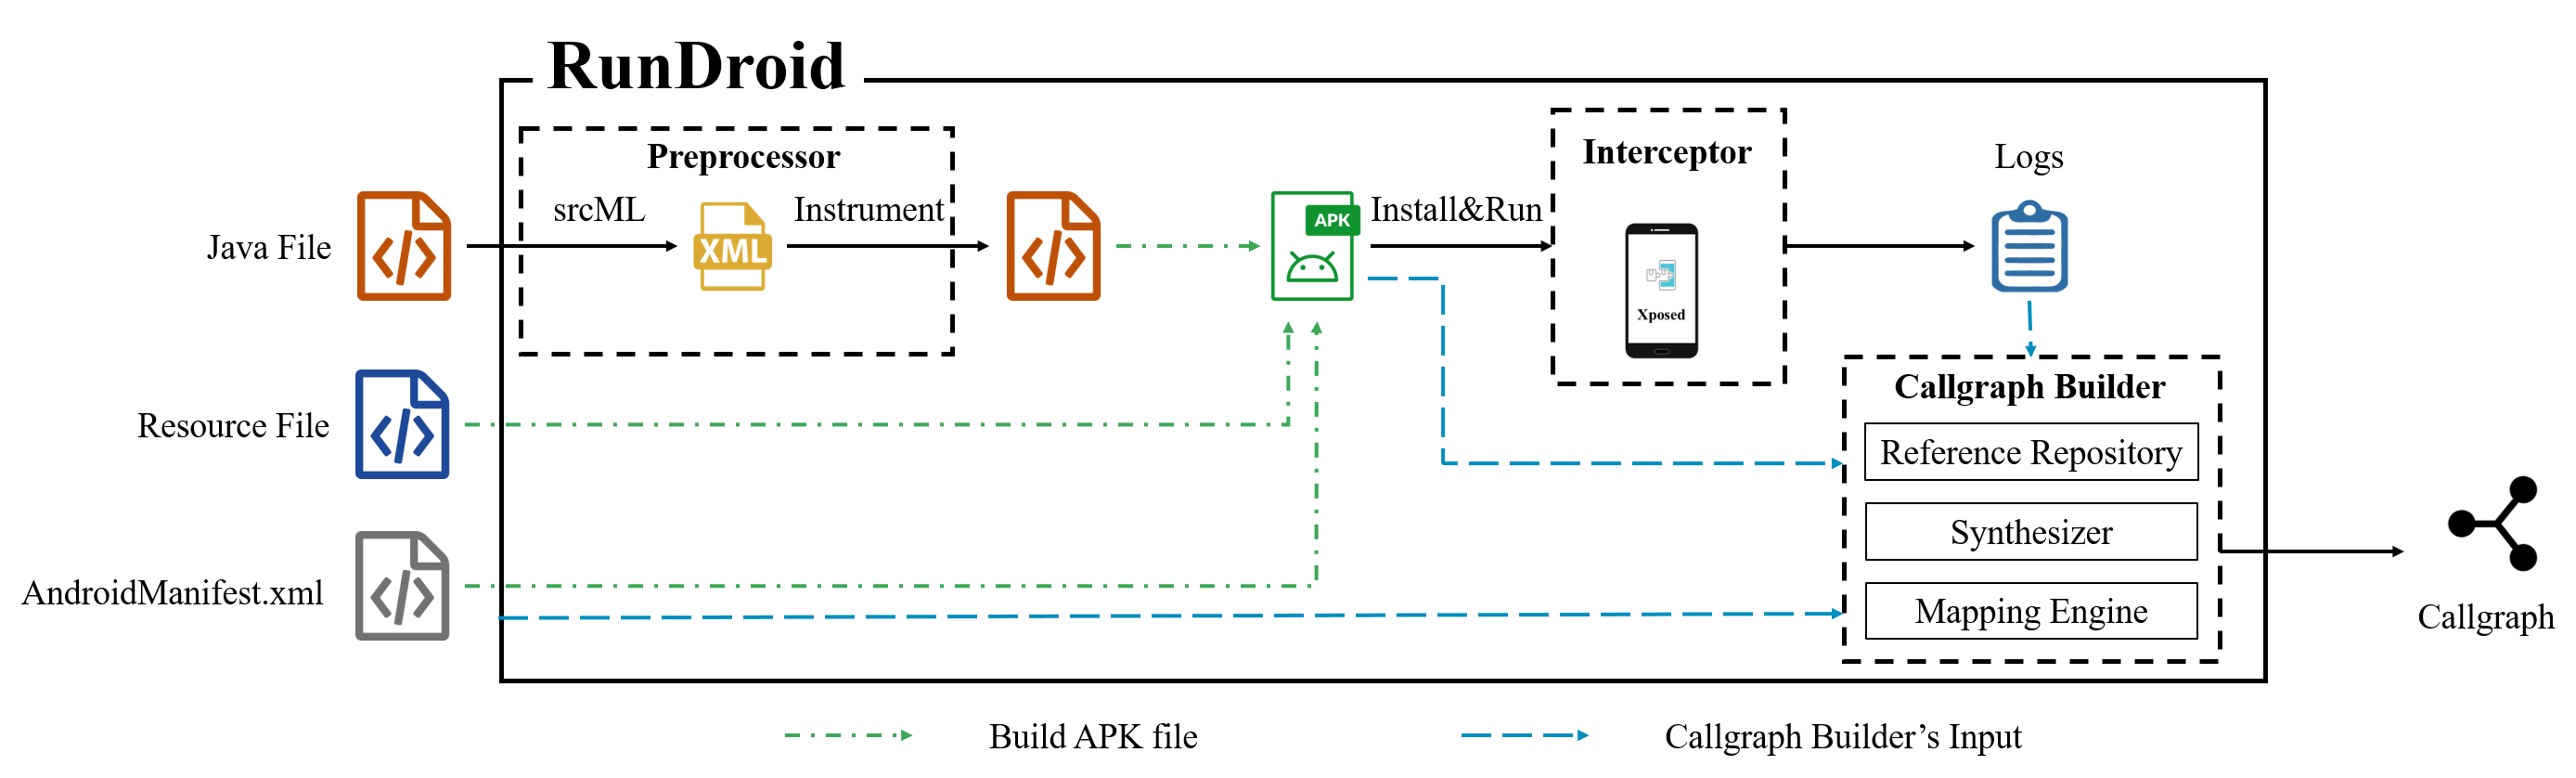
\includegraphics[keepaspectratio=true,width=1\linewidth]{Our-Approach.png}
\end{frame}
\subsection{How RunDroid works}
\begin{frame}
\frametitle{How RunDroid works}
\framesubtitle{Step 1:Capture application layer method calls\footnote{Application Layer Method Calls:the method defined by user/developer.}}

\textbf{Basic idea:}\newline
Log the target method's information before and after method's executed.

\textbf{Challenges:}\newline
The 64K reference limit(Emma) $\Longrightarrow$ Instrument on source code.

\textbf{Process:}\newline
Java file $\longrightarrow$ xml File $\longrightarrow$ xml file after instrumented $\longrightarrow$ The code with log methods.

\centering
\includegraphics[keepaspectratio=true,height=0.3\textheight]{example-image-c}

%插桩前后的代码对比
\end{frame}

\begin{frame}
\frametitle{How RunDroid works}
\framesubtitle{Step 2: Recover method calls between app and the Android framework}
\end{frame}

\begin{frame}
\frametitle{How RunDroid works}
\framesubtitle{Step 3: Build dynamic call graphs}
\end{frame}

\subsection{RunDroid for Visualization}
\begin{frame}
\frametitle{RunDroid for Visualization}
\begin{itemize}
	\item \textbf{The exact event sequences}, instead of all possible ones as the static analyzers do; 
	\item \textbf{The execution call graphs}, that are typically hard to capture with static analyzers; 
	\item \textbf{Related object information}, that assist in data flow analysis of static analyzers
\end{itemize}

\begin{columns}
	\column{0.56\textwidth}
	\begin{minipage}[c][0.4\textheight][c]{\linewidth}
		\centering
		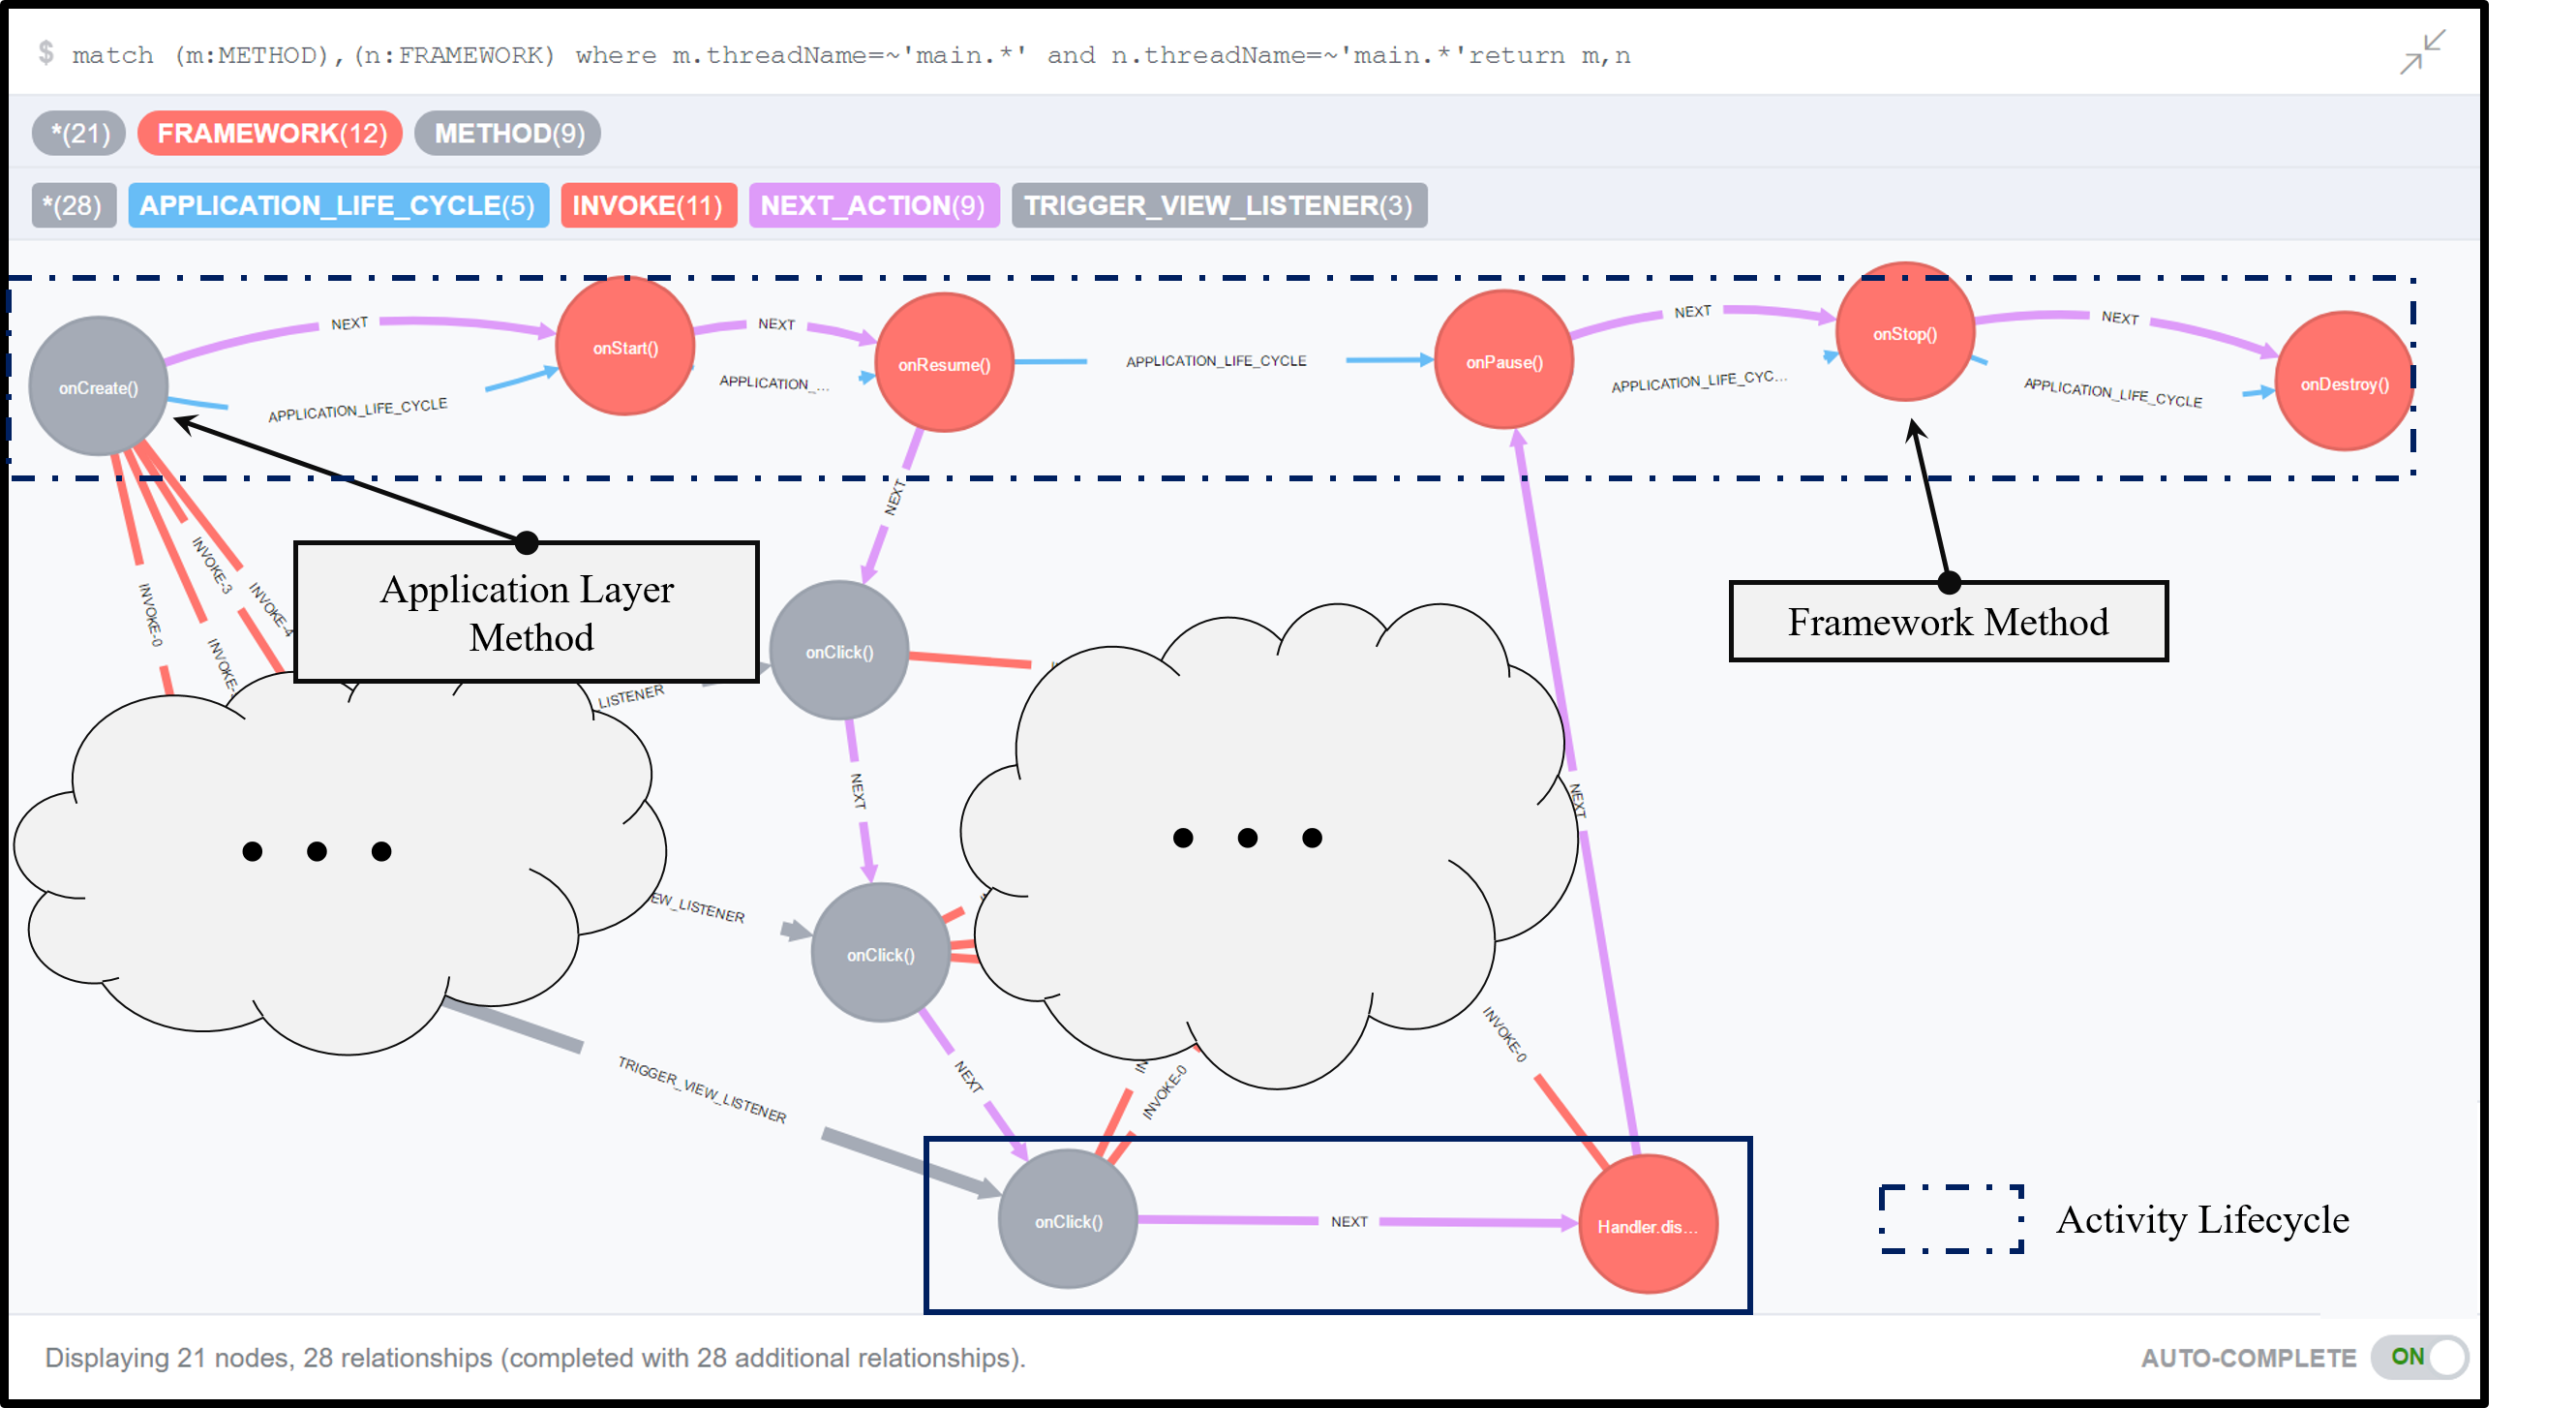
\includegraphics[width=\linewidth]{result-1.png}
	\end{minipage}
	\column{0.43\textwidth}
	\begin{minipage}[c][0.2\textheight][c]{\linewidth}
		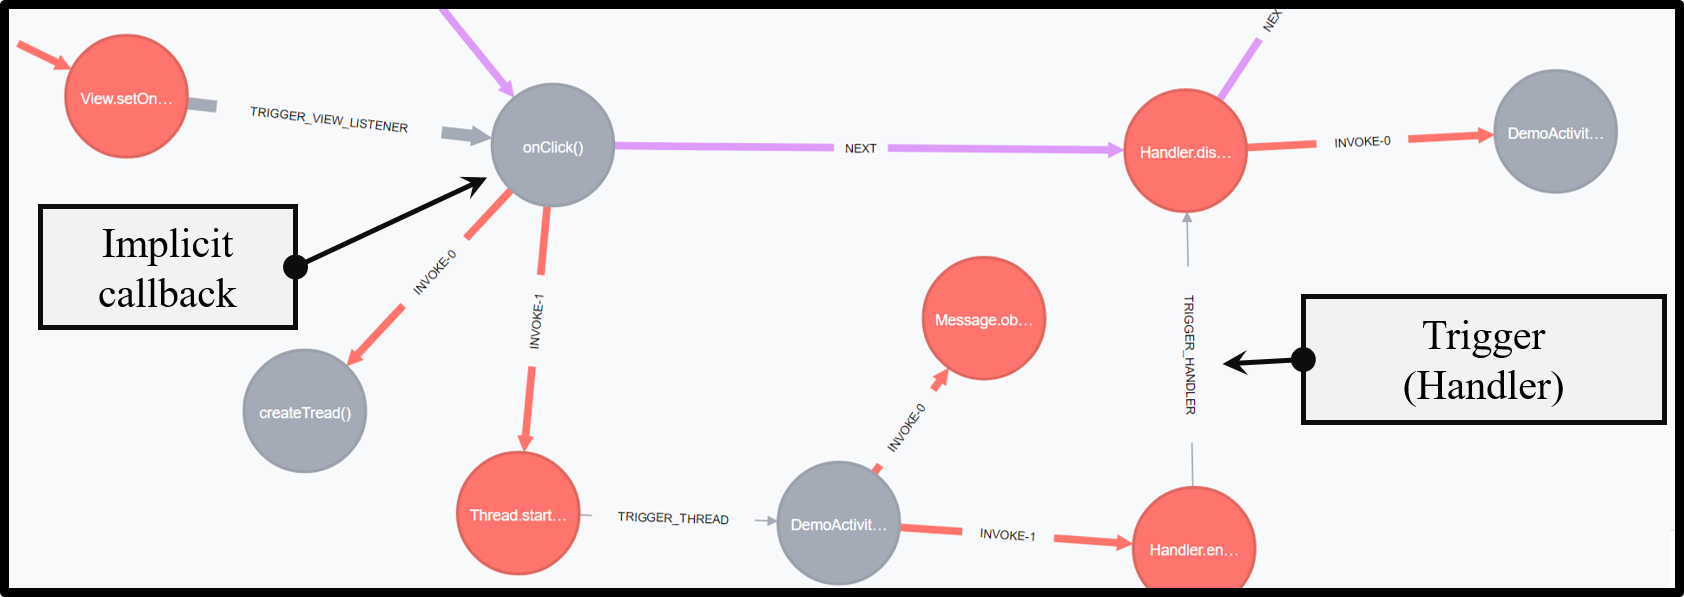
\includegraphics[width=\linewidth]{result-2.png}
	\end{minipage}
	\begin{minipage}[c][0.2\textheight][c]{\linewidth}
		\centering
		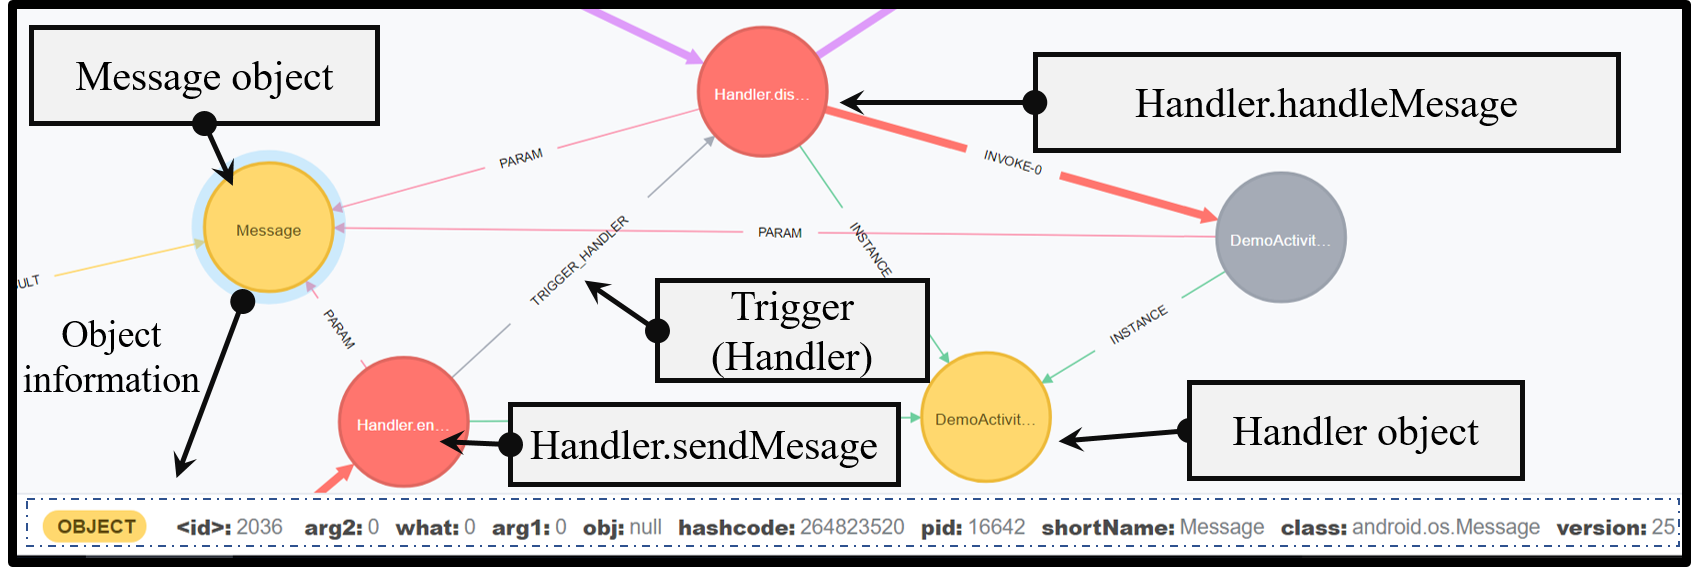
\includegraphics[width=\linewidth]{result-3.png}
	\end{minipage}
\end{columns}
\end{frame}

\subsection{RunDroid on fault localization}
\begin{frame}[fragile]
\frametitle{RunDroid on fault localization}

\begin{columns}
	
	\column{0.6\textwidth}
	To illustrate how the dynamic call graphs built by RunDroid assists fault localization techniques, we compare the estimation results using \textbf{the causal influence model} with or without RunDroid
	\column{0.45\textwidth}
	\begin{lstlisting}
void onClick(View v) {
  num = getNumber();
  if(v.getId() == R.id.btn1) {
    if( num == 0 ) {
      num=1;
    }
  }
  Thread t = createThread(v.getId());
  t.start();
}                  
TaskThread.run() {
  if(v.getId() == R.id.btn1) {
    loadData(num); /* FAULT */
  }
}       
\end{lstlisting}

	
\end{columns}
\end{frame}
\begin{frame}[fragile]
\frametitle{RunDroid on fault localization}


\begin{columns}
	
	\column{0.5\textwidth}
	% 
	Focs on Line 13:
	
	\centering
	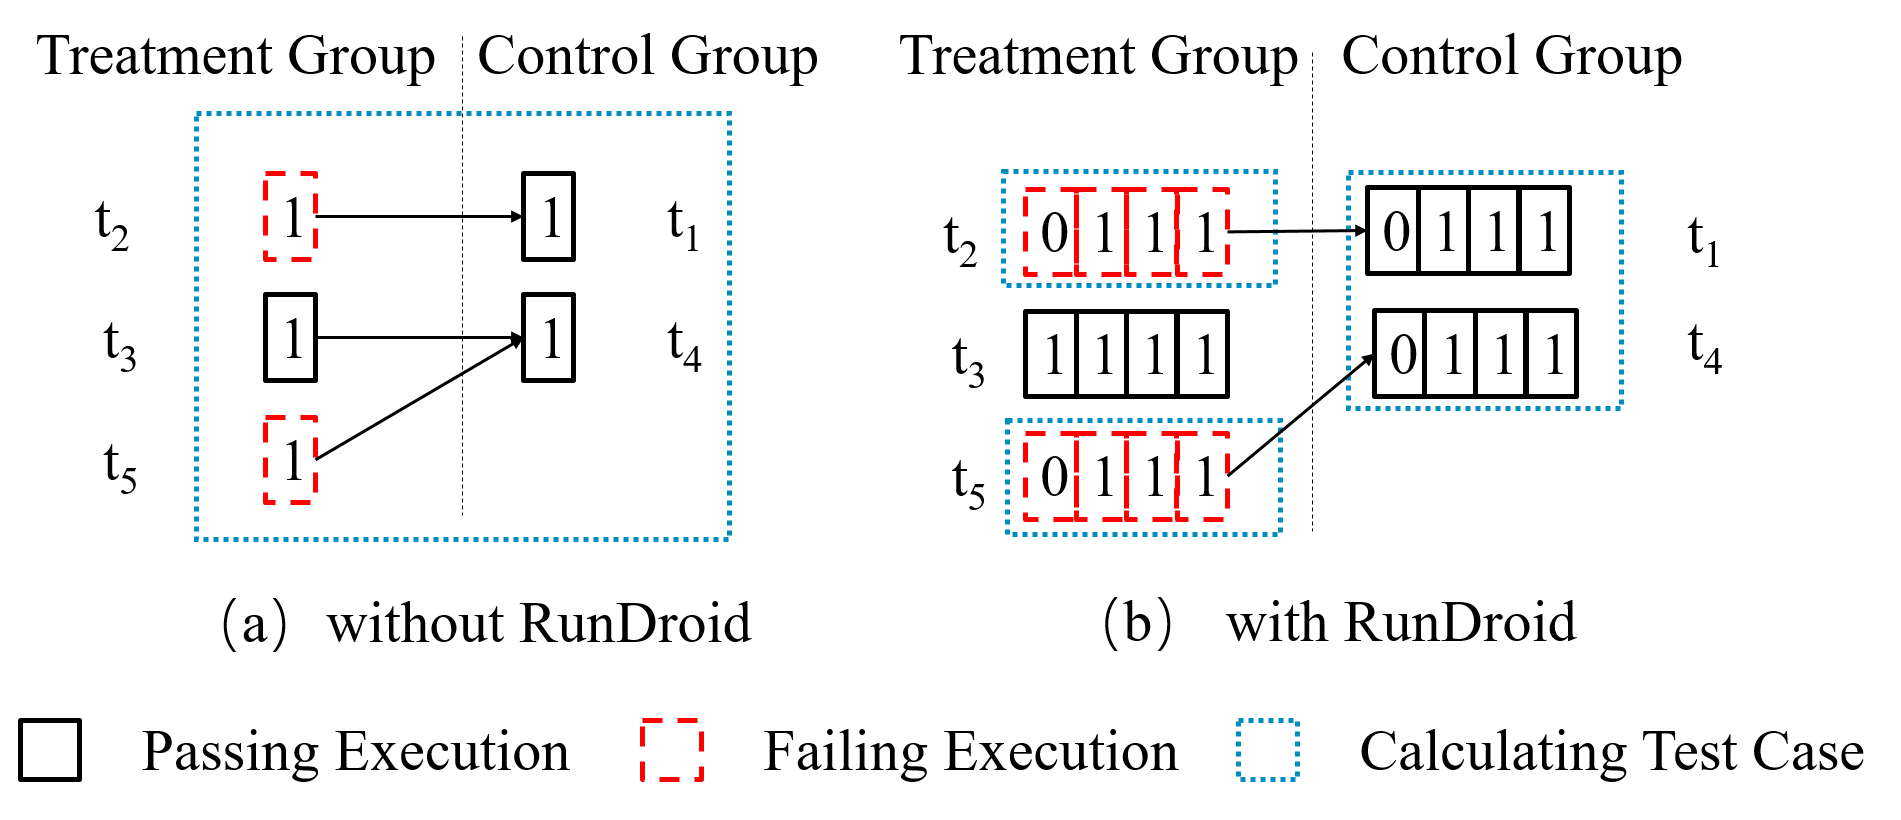
\includegraphics[keepaspectratio=true,width=\linewidth]{treatment.png}
	\column{0.5\textwidth}
\begin{lstlisting}
void onClick(View v) {
  num = getNumber();
  if(v.getId() == R.id.btn1) {
    if( num == 0 ) {
      num=1;
    }
  }
  Thread t = createThread(v.getId());
  t.start();
}                  
TaskThread.run() {
  if(v.getId() == R.id.btn1) {
    loadData(num); /* FAULT */
  }
}       
\end{lstlisting}
	
\end{columns}

\end{frame}
\begin{frame}
\frametitle{RunDroid on fault localization}
\begin{table}[h]
	\scriptsize	
	\caption{Comparing Results}
	\label{tab:result}
	\begin{tabular}{rl*{5} {|c}|c|c}
		
		&                    & $t_1$ & $t_2$ & $t_3$ & $t_4$ & $t_5$ &  $\tau$ &  $\tau'$ \\
		\hline
		1&void onClick(View v) \{                       &   &   &   &   &   &         \\
		2&\quad num = getNumber();                   & 1 & 1 & 1 & 1 & 1 &  NA  &  NA    \\
		3&\quad if(v.getId() == R.id.btn1) \{           & 1 & 1 & 1 & 1 & 1 &  NA    &  NA \\
		4&\quad \quad if( num == 0 ) \{                    & 0 & 1 & 1 & 0 & 1 & 0.67   & 0.67 \\
		5&\quad \quad \quad num=1;                         & 0 & 0 & 1 & 0 & 0 & -1.0  &-1\\
		6&\quad \quad \}                                   &   &   &   &   &   &             \\
		7&\quad   \}                                       &   &   &   &   &   &            \\
		8&\quad Thread t = createThread(v.getId());          & 1 & 1 & 1 & 1 & 1 & NA&  NA  \\
		9&\quad t.start();                                 & 1 & 1 & 1 & 1 & 1 & 0.67   & 0.67 \\
		10&\}                                              &   &   &   &   &   &             \\
		11&TaskThread.run() \{                             &   &   &   &   &   &       \\
		12&\quad if(v.getId() == R.id.btn1) \{                          & 1 & 1 & 1 & 1 & 1 &  NA   & 0.67 \\
		13&\quad \quad \textbf{loadData(num); /* FAULT */} & 0 & 1 & 1 & 0 & 1 & 0.67    & 1  \\
		14&\quad\}                                         &   &   &   &   &   &            \\
		15&\}                                              &   &   &   &   &   &           \\
		\hline
		&                                                  & 0 & 1 & 0 & 0 & 1 &            \\
	\end{tabular}
\end{table}

\end{frame}


\section{Customized work \& Furture work}
\begin{frame}
\frametitle{Customized work \& Furture work}
\textbf{Customized work}
\begin{itemize}
	\item customize the log output about object information
	\item add or remove Android framework methods to hook the methods' executions
	\item add or remove more method-trigger relationships in Call Graph 
\end{itemize}

\textbf{Furture work}
\begin{itemize}
\item add control flow unit into the call graph
\end{itemize}
\end{frame}

\end{document}